\documentclass{article}

\usepackage{graphicx} % Required for the inclusion of images
\usepackage{amsmath} % Required for some math elements
\usepackage{listings}
\usepackage{verbatim}
\usepackage{float}

\usepackage{tabularx}
\usepackage{colortbl}
\usepackage{hhline}

\topmargin0.0cm
\headheight0.0cm
\headsep0.0cm
\oddsidemargin0.0cm
\textheight23.0cm
\textwidth16.5cm
\footskip1.0cm
\setlength{\parindent}{0pt}
\setlength{\parskip}{0.7em}

\title{Clusters and Classification Boundaries} % Title
\author{SYDE 372 - Lab 1} % Author name
\date{February 12th, 2017} % Date for the report

\begin{document}

\maketitle

\begin{center}
\begin{tabular}{l r}
Group Members: & Krishn Ramesh - 20521942 \\ % Partner names
& Brady Kieffer - 20517665 \\
& Ramandeep Farmaha - 20516974 \\
& Shubam Mehta - 20483061\\
Instructor: & Professor Wong % Instructor/supervisor
\end{tabular}
\end{center}




\section{Introduction}

Clustering and classifying data points is a fundamental skill in pattern recognition. Lab 1 provides a hands-on introduction to generating different kinds of decision boundaries, as well as evaluating and comparing their performance. Two cases with true statistics (mean, covariance matrices) for the classes in each case were provided. The initial setup work in generating the sampled data involved bivariate normal distributions subject to orthonormal transformations. Different distance measures were used to construct decision boundaries including MED, GED, MAP, NN and kNN. Lastly, the performance of each distance measure was analyzed and compared. Overall, Lab 1 provided valuable insight into the use of orthonormal transformations, decision boundaries and classification errors to solve practical problems.



\section{Generating Clusters}
Five classes were considered in this lab, split up into two cases. All the classes followed the following bivariate Gaussian distribution parameters:

CASE 1:
\begin{gather*}
\text{Class A:}\quad N_A = 200 \quad \mu_A = \begin{bmatrix} 5 & 10 \end{bmatrix}^T \quad \Sigma_A = \begin{bmatrix} 8 & 0 \\ 0 & 4  \end{bmatrix} \\
\text{Class B:}\quad N_B = 200 \quad \mu_B = \begin{bmatrix} 10 & 15 \end{bmatrix}^T \quad \Sigma_B = \begin{bmatrix} 8 & 0 \\ 0 & 4  \end{bmatrix}
\end{gather*}

CASE 2:
\begin{gather*}
\text{Class C:}\quad N_C = 100 \quad \mu_C = \begin{bmatrix} 5 & 10 \end{bmatrix}^T \quad \Sigma_C = \begin{bmatrix} 8 & 4 \\ 4 & 40  \end{bmatrix} \\
\text{Class D:}\quad N_D = 200 \quad \mu_D = \begin{bmatrix} 15 & 10 \end{bmatrix}^T \quad \Sigma_D = \begin{bmatrix} 8 & 0 \\ 0 & 8  \end{bmatrix} \\
\text{Class E:}\quad N_E = 150 \quad \mu_E = \begin{bmatrix} 10 & 5 \end{bmatrix}^T \quad \Sigma_D = \begin{bmatrix} 10 & -5 \\ -5 & 20  \end{bmatrix}
\end{gather*}

The clusters were generated using the \verb|randn| function provided by \verb|MATLAB|. First, data was generated with a mean of zero and a variance of one. The provided covariance matrix for each class was diagonalized using Cholesky factorization provided within the \verb|chol| function. The data was then transformed by first multiplying the sampled points by this diagonalized matrix and then adding the class mean to each row. The provided function \verb|bivariate_normal| was used to generate samples for each of the classes provided in the lab. This produced data centered about the provided class mean with their respective covariances.

After generating sample data for each of the classes, they were plotted as a scatter plot with a unit standard deviation contour.

\begin{figure}[H]
\caption{Plot of Case 1}
\centering
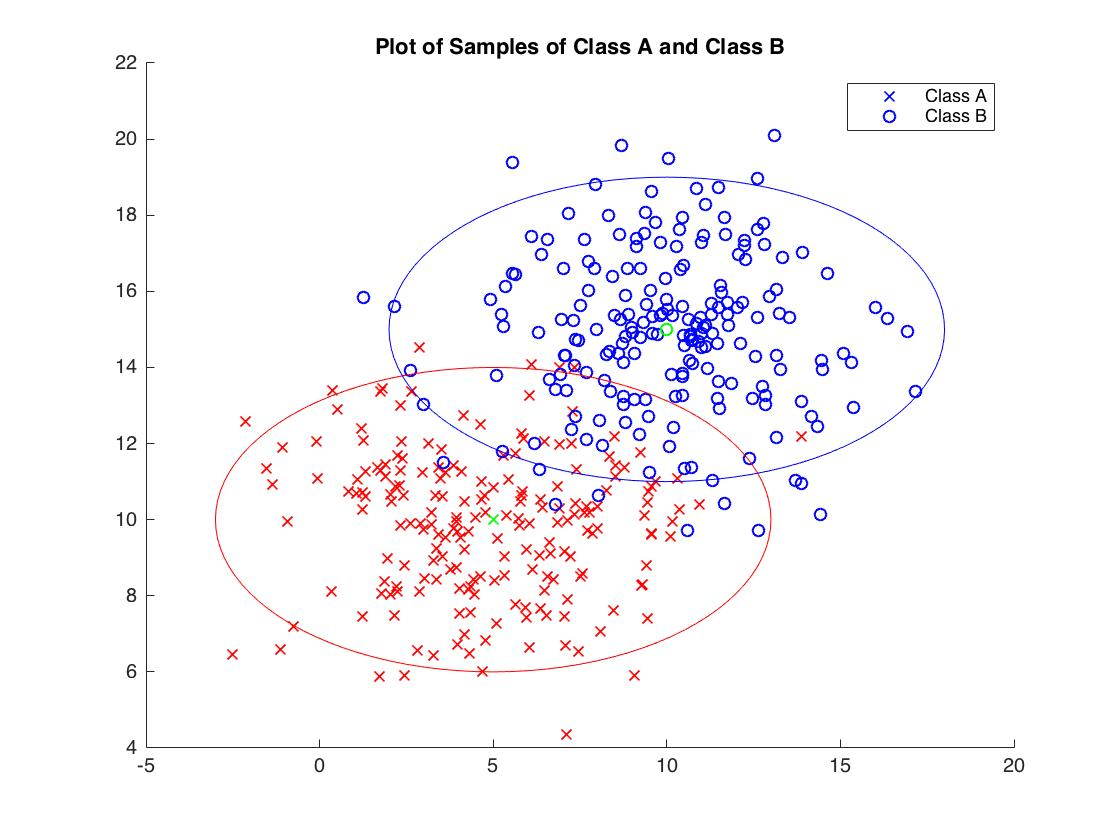
\includegraphics[width=0.5\textwidth]{Case1ScatterPlot}
\label{fig:Case1Scatter}
\end{figure}

\begin{figure}[H]
\caption{Plot of Case 2}
\centering
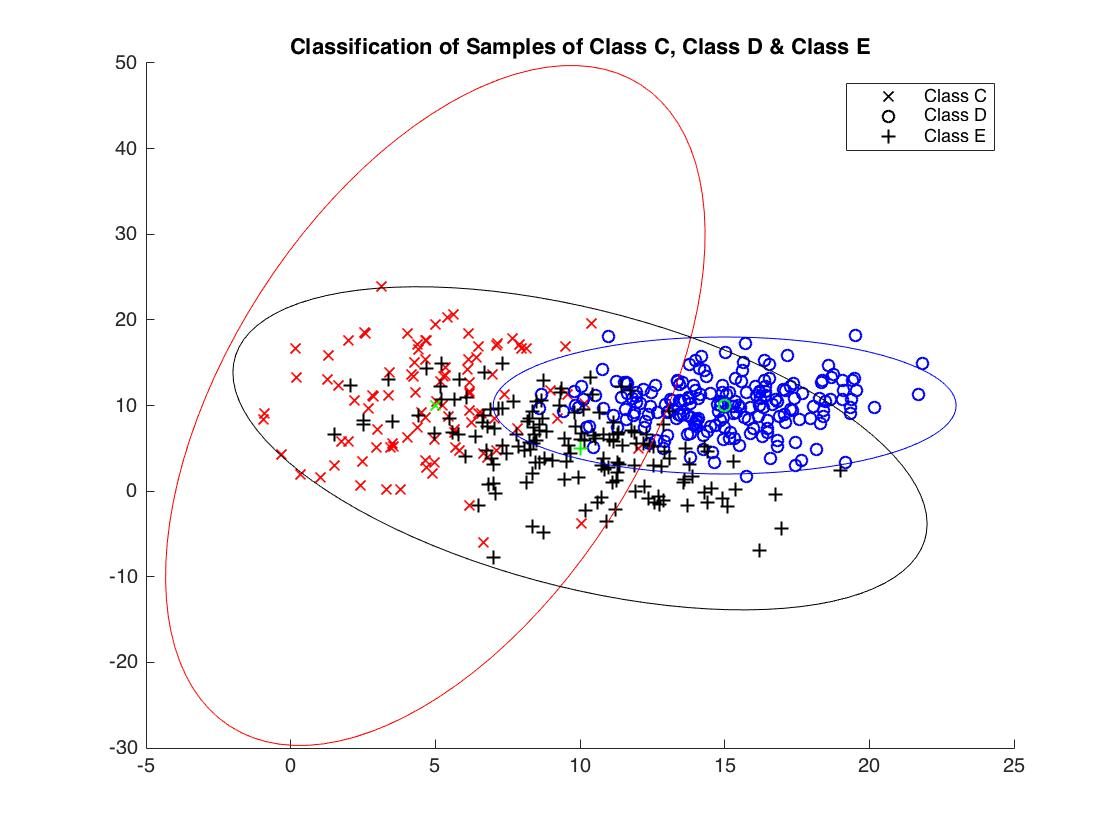
\includegraphics[width=0.5\textwidth]{Case2ScatterPlot}
\label{fig:Case2Scatter}
\end{figure}

The means of all the classes are plotted in green. The unit standard deviation contours were plotted using the \verb|plot_ellipse| function. The lengths of the major and minor axes of the ellipse were determined by the square root of the 2 eigenvalues of each cluster. The angle of the ellipses was determined by taking the $arctan(\cdot)$ of the ratio of the eigenvector elements of each cluster.

Visually, the unit contour contains approximately 68\% of the data, as the contour represents 1 standard deviation from the mean. The unit contour is centered at the mean of each class and follows the shape of the data; its major axis is aligned with the direction of greatest variance of the data, while its minor axis is aligned with the direction of least variance.


\section{Classifiers and Error Analysis}

All of the classifiers were approached numerically and implemented in \verb|MATLAB|. A 2D grid of points was created for each case and run through all of the classifiers to classify each point in the grid. The decision boundaries were then plotted on top of the sample data using contour plots.

The errors for each classifier were also analyzed. The experimental error rate $P(\epsilon)$ for each case, was calculated as the number of samples classified wrong as a percentage of the total number of samples.
$$
P(\epsilon) = \frac{\text{samples classified wrong}}{\text{{total number of samples}}}
$$
The confusion matrix for each classifier was also produced to analyze its performance in further detail.

\subsection{Minimum Euclidean Distance (MED)}
The idea behind a Minimum Euclidean Distance classifier is to measure the Euclidean distance between the data point to be classified and the mean of all available classes. The data point then gets classified to the class with the lowest Euclidean Distance to its mean. The MED to each class mean was obtained using the following:
\[d_E(\bar{x}, \bar{\mu}_{k}) = [(\bar{x} - \bar{\mu}_{k})^{T}(\bar{x} - \bar{\mu}_{k})]^{1/2}\]

where $d_E(\bar{x}, \bar{\mu}_k)$ represents the MED for data point $\bar{x}$ to class mean $\bar{\mu}_{k}$.

The MED Classifier was implemented using \verb|MATLAB|. The mathematical form used for implementation was:
\[[(\bar{x} - \bar{\mu}_{A})^{T}(\bar{x} - \bar{\mu}_{A})]^{1/2} <
    [(\bar{x} - \bar{\mu}_{B})^{T}(\bar{x} - \bar{\mu}_{B})]^{1/2}\]
where:
\begin{itemize}
    \item {$\bar{x}$ was the data point to be classified.}
    \item {$\bar{\mu}_k$ was the mean of class k.}
\end{itemize}


Once the MED was computed for each data point, it was classified to its respective class and the decision boundary separated each class. The function specified above to calculate the MED lies in the \verb|MED.m| file. Running the function on the classes provided in Case 1 generate the figure shown below in Figure 3.

\begin{figure}[H]
\caption{Plot of Case 1 with MED Classifier (white line)}
\centering
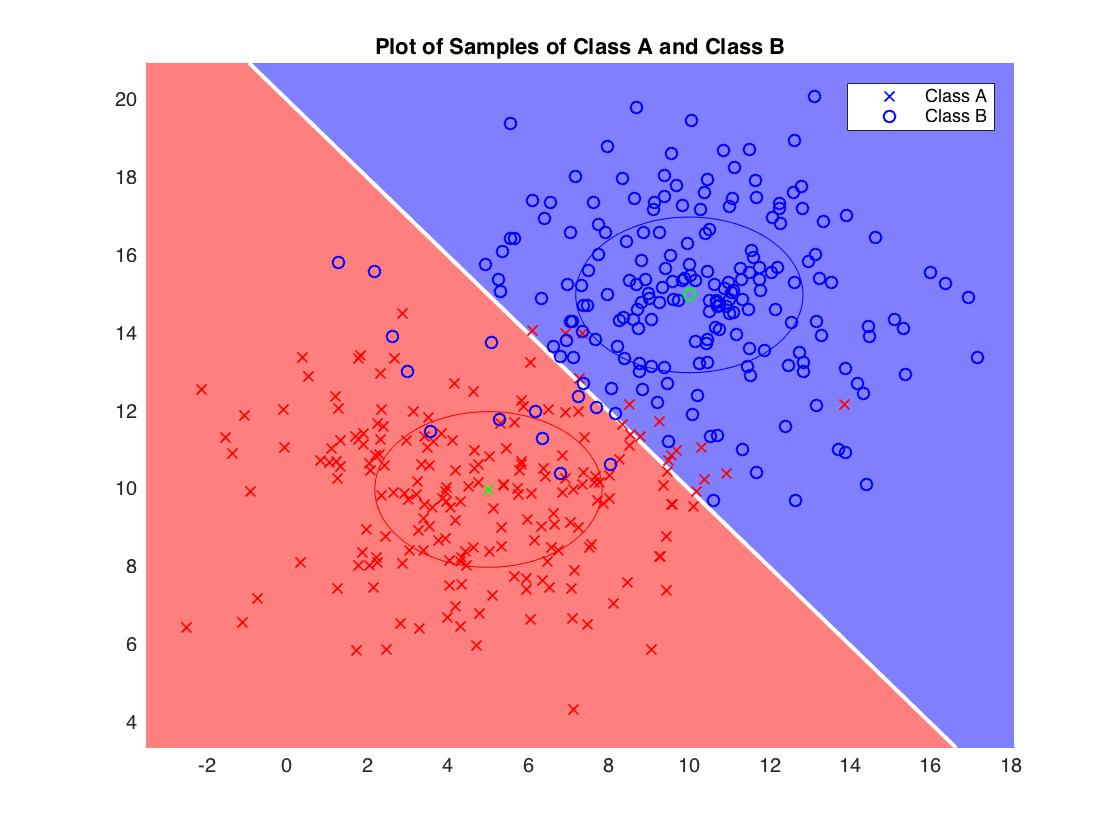
\includegraphics[width=0.5\textwidth]{Case1MED}
\label{fig:Case1_MED}
\end{figure}

The MED classifier results were as expected with the decision boundary being a diagonal line between both classes. The MED line was a perpendicular bisector of the line between the two means.

For case 1, the experimental error rate was:
\[P(\epsilon) = 0.0725\]
A confusion matrix of the results can be viewed in table 1 below.

\begin{table}[H]
    \centering
    \begin{tabular}{c|c c|c|}
        & \multicolumn{2}{c|}{\textbf{Predicted}} \\
        \textbf{Actual} & \textbf{A} & \textbf{B} & \textbf{Totals} \\
        \hline
        \textbf{A} & 184 \cellcolor[gray]{.8} & 16 & 200\\
        \textbf{B} & 13 & 187 \cellcolor[gray]{.8} & 200\\\hline
        \textbf{Totals} & 197 & 203\\
        \cline{1-3}
    \end{tabular}
    \caption{Confusion matrix for Case 1 with MED.}
    \label{tab:Case1_MED_error}
\end{table}

Case 2 consisted of 3 different classes and the same classifier function was used for each pair of classes. The result for case 2 is shown below in Figure 4.

\begin{figure}[H]
\caption{Plot of Case 2 with MED Classifier (white lines)}
\centering
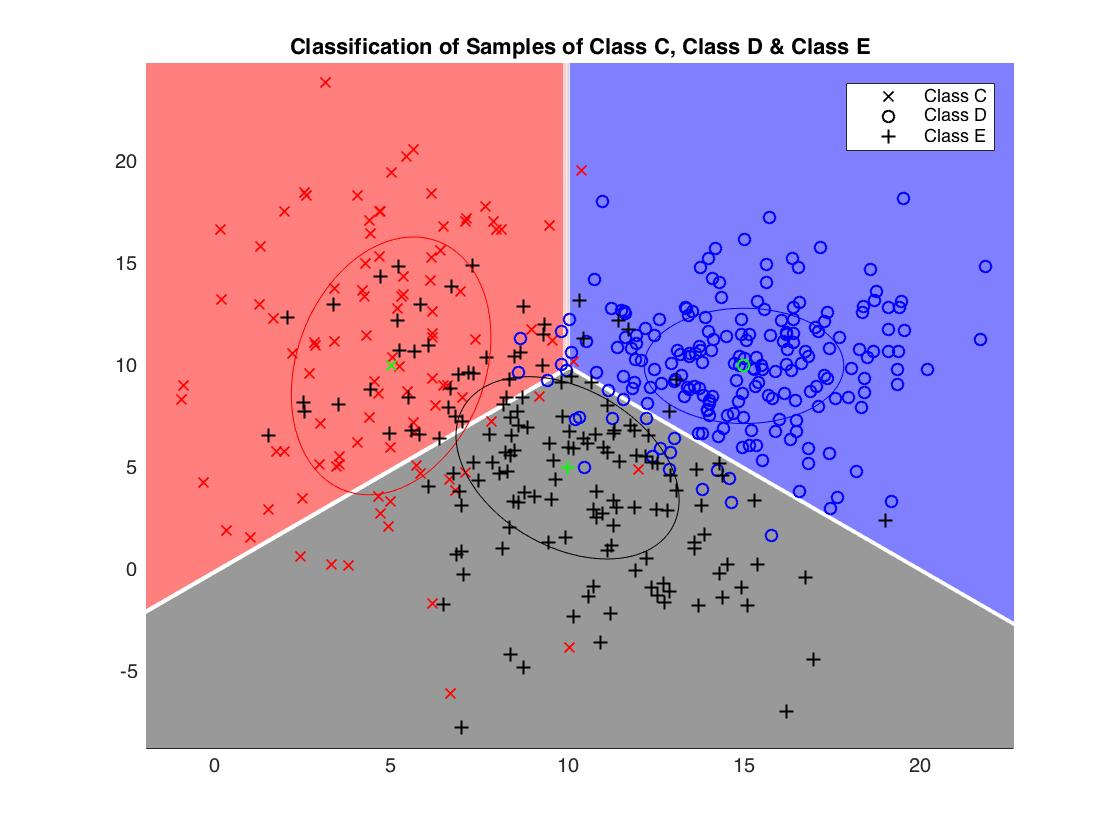
\includegraphics[width=0.5\textwidth]{Case2MED}
\label{fig:Case2_MED}
\end{figure}

The results were once again linear as expected but there were still some points past the decision boundaries due to the error. For case 2, the experimental error rate was:
\[P(\epsilon) = 0.1933\]
which as expected was higher than case 1 due to a higher number of classes. The confusion matrix for case 2 is shown below in table 2.

\begin{table}[H]
    \centering
    \begin{tabular}{c|c c c|c|}
        & \multicolumn{3}{c|}{\textbf{Predicted}} \\
        \textbf{Actual} & \textbf{C} & \textbf{D} & \textbf{E} & \textbf{Totals} \\
        \hline
        \textbf{C} & 80 \cellcolor[gray]{.8} & 2 & 18 & 100 \\
        \textbf{D} & 4 & 177 \cellcolor[gray]{.8} & 19 & 200\\
        \textbf{E} & 37 & 7 & 106 \cellcolor[gray]{.8} & 150\\\hline
        \textbf{Totals} & 121 & 186 & 143\\
        \cline{1-4}

    \end{tabular}
    \caption{Confusion matrix for Case 2 with MED.}
    \label{tab:Case2_MED_error}
\end{table}

\subsection{Generalized Euclidean Distance (GED)}
The GED classifier was implemented using \verb|MATLAB|. The mathematical form used for implementation was:
\[(\bar{x} - \bar{\mu}_{A})^{T}\Sigma^{-1}_{A}(\bar{x} - \bar{\mu}_{A}) <
    (\bar{x} - \bar{\mu}_{B})^{T}\Sigma^{-1}_{B}(\bar{x} - \bar{\mu}_{B})\]
Where:
\begin{itemize}
    \item {$\bar{x}$ was the data to be classified.}
    \item {$\bar{\mu}_C$ was the class mean.}
    \item {$\Sigma_{C}$ was the covariance matrix for the class.}
\end{itemize}

Classifying whether a given point belonged to either class $A$ or $B$ was trivial by rearranging the inequality to obtain the following:
\[(\bar{x} - \bar{\mu}_{A})^{T}\Sigma^{-1}_{A}(\bar{x} - \bar{\mu}_{A}) -
    (\bar{x} - \bar{\mu}_{B})^{T}\Sigma^{-1}_{B}(\bar{x} - \bar{\mu}_{B}) < 0\]

 If the difference was less than zero then the point was chosen to belong to class $A$. If it was greater than zero then class $B$ was chosen. The decision boundary would then lie where the difference between the distances was zero. A function to calculate the GED between two classes was created and provided within the \verb|GED.m| folder. Running \verb|GED| on the classes provided within Case 1 generated the results within figure \ref{fig:Case1_GED}.

\begin{figure}[H]
    \caption{Plot of decision boundary for GED on Case 1.}
    \centering
    \includegraphics[width=0.5\textwidth]{Case1_GED}
    \label{fig:Case1_GED}
\end{figure}

The GED classifier behaved as expected with the decision boundary being drawn between the two standard deviation contours. It should also be noted that the decision boundary was a straight line due to the features being uncorrelated.

For Case 1 with the GED classifier the probability of error was:
\[P(\epsilon) = 0.0550\]
And a confusion matrix of the results can be viewed within table \ref{tab:Case1_GED_error}.

\begin{table}[H]
    \centering
    \begin{tabular}{c|c c|c|}
        & \multicolumn{2}{c|}{\textbf{Predicted}} \\
        \textbf{Actual} & \textbf{A} & \textbf{B} & \textbf{Totals} \\
        \hline
        \textbf{A} & 192 \cellcolor[gray]{.8} & 8 & 200\\
        \textbf{B} & 14 & 186 \cellcolor[gray]{.8} & 200\\\hline
        \textbf{Totals} & 206 & 194\\
        \cline{1-3}
    \end{tabular}
    \caption{Confusion matrix for Case 1 with GED.}
    \label{tab:Case1_GED_error}
\end{table}

The results of the GED classifier on Case 2 can be viewed within figure \ref{fig:Case2_GED}. Again the classifier behaved as expected with the decision boundaries being non-linear and passing through any intersection of the standard deviation contours.

\begin{figure}[H]
    \caption{Plot of decision boundary for GED on Case 2.}
    \centering
    \includegraphics[width=0.5\textwidth]{Case2_GED}
    \label{fig:Case2_GED}
\end{figure}

For Case 2 with the GED classifier the observed probability of error was:
\[P(\epsilon) = 0.1756\]

And a confusion matrix can be viewed within table \ref{tab:Case2_GED_error}

\begin{table}[H]
    \centering
    \begin{tabular}{c|c c c|c|}
        & \multicolumn{3}{c|}{\textbf{Predicted}} \\
        \textbf{Actual} & \textbf{C} & \textbf{D} & \textbf{E} & \textbf{Totals} \\
        \hline
        \textbf{C} & 91 \cellcolor[gray]{.8} & 0 & 9 & 100 \\
        \textbf{D} & 3 & 169 \cellcolor[gray]{.8} & 28 & 200\\
        \textbf{E} & 35 & 4 & 111 \cellcolor[gray]{.8} & 150\\\hline
        \textbf{Totals} & 129 & 173 & 148\\
        \cline{1-4}

    \end{tabular}
    \caption{Confusion matrix for Case 2 with GED.}
    \label{tab:Case2_GED_error}
\end{table}

\subsection{Maximum A Posteriori (MAP)}
The MAP classifier is a powerful classifier which assigns an unknown pattern as belonging to a class based on the highest \textit{a posteriori} class probabilities i.e. $P(A|\bar{x})$. It makes the reasonable assumption that the class with the highest probability given the particular point $\bar{x}$ is the class that $\bar{x}$ belongs to. Mathematically:

$$
\bar{x} \in A \quad \text{iff} \quad P(A|\bar{x}) > P(B|\bar{x})
$$

This can be simplified using Bayes Rule, assuming Normal distributions for both classes and using log-likelihood form to obtain the decision boundary:

$$
(\bar{x}-\bar{\mu}_B)^T \Sigma_B^{-1} (\bar{x}-\bar{\mu}_B) - (\bar{x} -\bar{\mu}_A)^T \Sigma_A^{-1} (\bar{x}-\bar{\mu}_A) = 2\ln{\frac{P(B)}{P(A)}}+\ln{\frac{|\Sigma_A|}{|\Sigma_B|}}
$$

When coding it up in \verb|MATLAB|, the classifier was represented by:

$$
\bar{x}^T Q_0 \bar{x} + Q_1\bar{x} + Q2 + 2Q3 + Q4
$$
where:
\begin{gather*}
Q_0 = \Sigma_A^{-1} - \Sigma_B^{-1} \\
Q_1 = 2[\bar{\mu}_B^T \Sigma_B^{-1} - \bar{\mu}_A^T \Sigma_A^{-1}] \\
Q_2 = \bar{\mu}_A^T \Sigma_A^{-1} \bar{\mu}_A - \bar{\mu}_B^T \Sigma_B^{-1} \bar{\mu}_B \\
Q_3 = \ln{\frac{P(B)}{P(A)}} \\
Q_4 = \ln{\frac{|\Sigma_A|}{|\Sigma_B|}}
\end{gather*}

The prior probabilities were proportional to the number of samples in each class using the true class statistics given in section 1. If the classifier value for a point was negative, it belonged to class A, otherwise it belonged to class B. Points with a MAP classifier value of 0 were on the decision boundary.

Running a MAP classifier through the sample data for case 1 (with class A and class B) produced a line separating the classes.

\begin{figure}[H]
\caption{Plot of Case 1 with MAP Classifier (black line)}
\centering
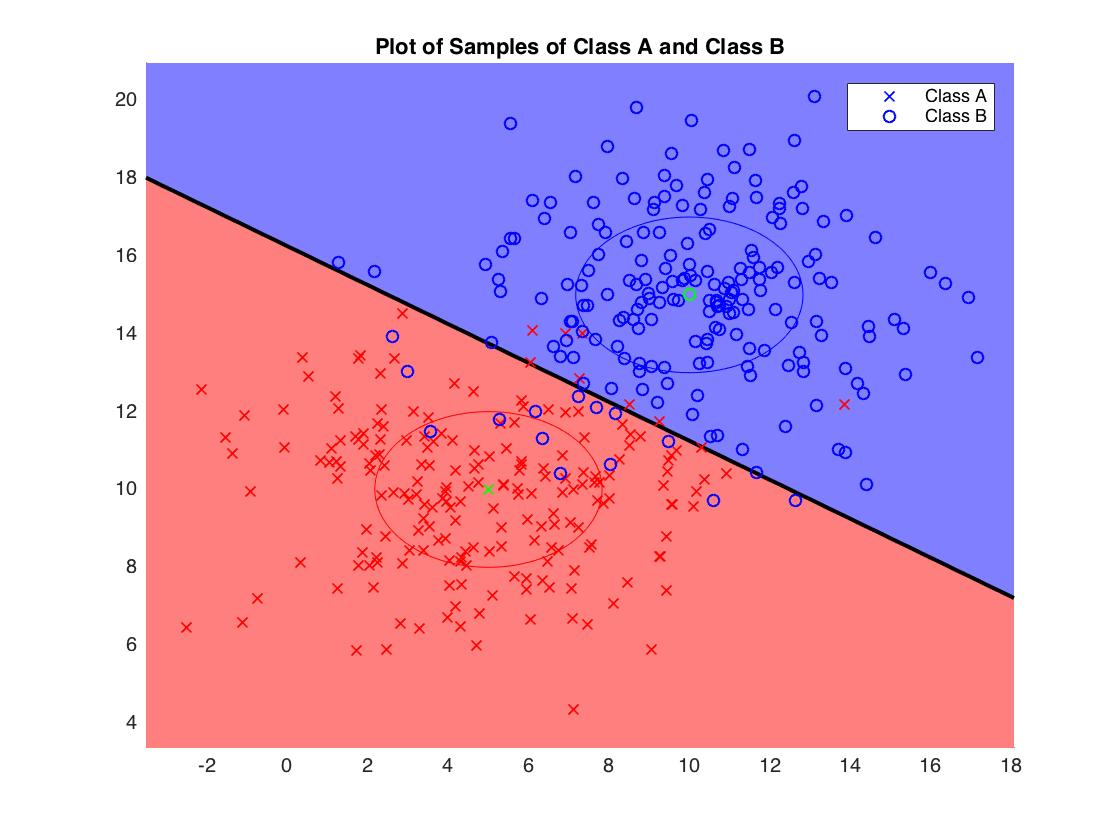
\includegraphics[width=0.5\textwidth]{Case1MAP}
\label{fig:Case1_MAP}
\end{figure}

Although the MAP classification was not perfect, it is the optimal decision boundary considering the posterior probabilities. It is noteworthy that the MAP decision line is not perpendicular to the line connecting the means of the two classes.

The experimental error rate for case 1 was:
$$
P(\epsilon) = 0.0550
$$

The confusion table for case 1 can be seen below.

\begin{table}[H]
    \centering
    \begin{tabular}{c|c c|c|}
        & \multicolumn{2}{c|}{\textbf{Predicted}} \\
        \textbf{Actual} & \textbf{A} & \textbf{B} & \textbf{Totals} \\
        \hline
        \textbf{A} & 192 \cellcolor[gray]{.8} & 8 & 200\\
        \textbf{B} & 14 & 186 \cellcolor[gray]{.8} & 200\\\hline
        \textbf{Totals} & 206 & 194\\
        \cline{1-3}
    \end{tabular}
    \caption{Confusion Table for Case 1 with MAP}
    \label{tab:Case1_MAP_error}
\end{table}

Case 2 with 3 overlapping classes was more complicated, but the MAP classifier still handled it well.

\begin{figure}[H]
\caption{Plot of Case 2 with MAP Classifier (black curve)}
\centering
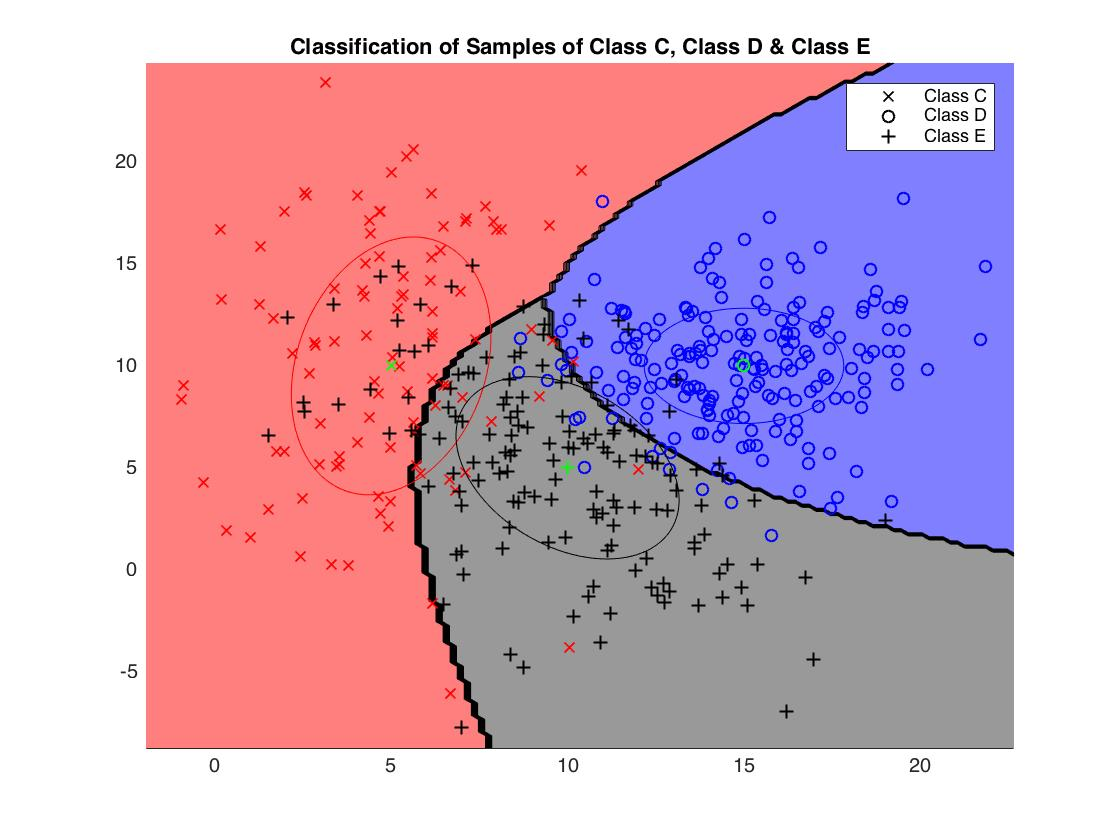
\includegraphics[width=0.5\textwidth]{Case2MAP}
\label{fig:Case2_MAP}
\end{figure}

This time the decision boundary was no longer linear, but curved. The MAP classifier nicely separated all 3 classes with most of the samples being classified correctly.

The experimental error rate for case 2 was:
$$
P(\epsilon) = 0.1511
$$
This was higher than the error rate in case 1 but that was expected due to the more complex nature of this problem. There was a lot of overlap among the 3 classes, and they were definitely not linearly separable. Still, the MAP classifier did an admirable job.

The confusion table for case 2 goes over the classification in more detail.
\begin{table}[H]
    \centering
    \begin{tabular}{c|c c c|c|}
        & \multicolumn{3}{c|}{\textbf{Predicted}} \\
        \textbf{Actual} & \textbf{C} & \textbf{D} & \textbf{E} & \textbf{Totals} \\
        \hline
        \textbf{C} & 84 \cellcolor[gray]{.8} & 1 & 15 & 100 \\
        \textbf{D} & 1 & 182 \cellcolor[gray]{.8} & 17 & 200\\
        \textbf{E} & 21 & 13 & 116 \cellcolor[gray]{.8} & 150\\\hline
        \textbf{Totals} & 106 & 196 & 148\\
        \cline{1-4}
    \end{tabular}
    \caption{Confusion matrix for Case 2 with MAP}
    \label{tab:Case2_MAP_error}
\end{table}


\subsection{Nearest Neighbor (NN) and k-Nearest Neighbor (kNN)}
The Nearest Neighbor and k-Nearest Neighbor classifiers differ from the rest of the classifiers discussed in this report primarily because they utilize all elements of sample classes, rather than the mean and covariance.

The basic idea of the NN classifier is that for a given point $P$, the Euclidean distances between $P$ and all points within sample classes $A$ and $B$ are computed. Point $P$ is then assigned to the class that contains the closest point to $P$. This can be summarized in the following mathematical expression:
\begin{equation}
    z_k(x) = \bar{x}_k : d_E(\bar{x}, \bar{x}_k) = min_id_E(\bar{x}, \bar{x}_i) \forall\bar{x}_i \in c_k
\end{equation}

Where:
\begin{itemize}
    \item{$z_k(x)$ is the potential class that the point belongs to}
    \item{$\bar{x_k}$ is the closest sample to the point $\bar{x}$}
    \item{$c_k$ is the sample class}
\end{itemize}

This can be translated to determining the decision boundary between two classes in the following method:
\begin{enumerate}
    \item{Iterate over each point in the generated 2D grid}
    \item{For each point, compute the distances between all sample points in both classes and determine the nearest neighbor for both classes}
    \item{Assign the value of that point to the difference of the two distances}
\end{enumerate}

The method above generates a contour map that indicates the regions for either class. If the value of a point is negative, it belongs to class $A$ and class $B$ if it is positive. If the value of a point is 0, this indicates that no decision can be made about which class that point belongs to, i.e. it forms the boundary of the two classes.

\begin{figure}[H]
\caption{Plot of Case 1 with NN Classifier (Black Curves)}
\centering
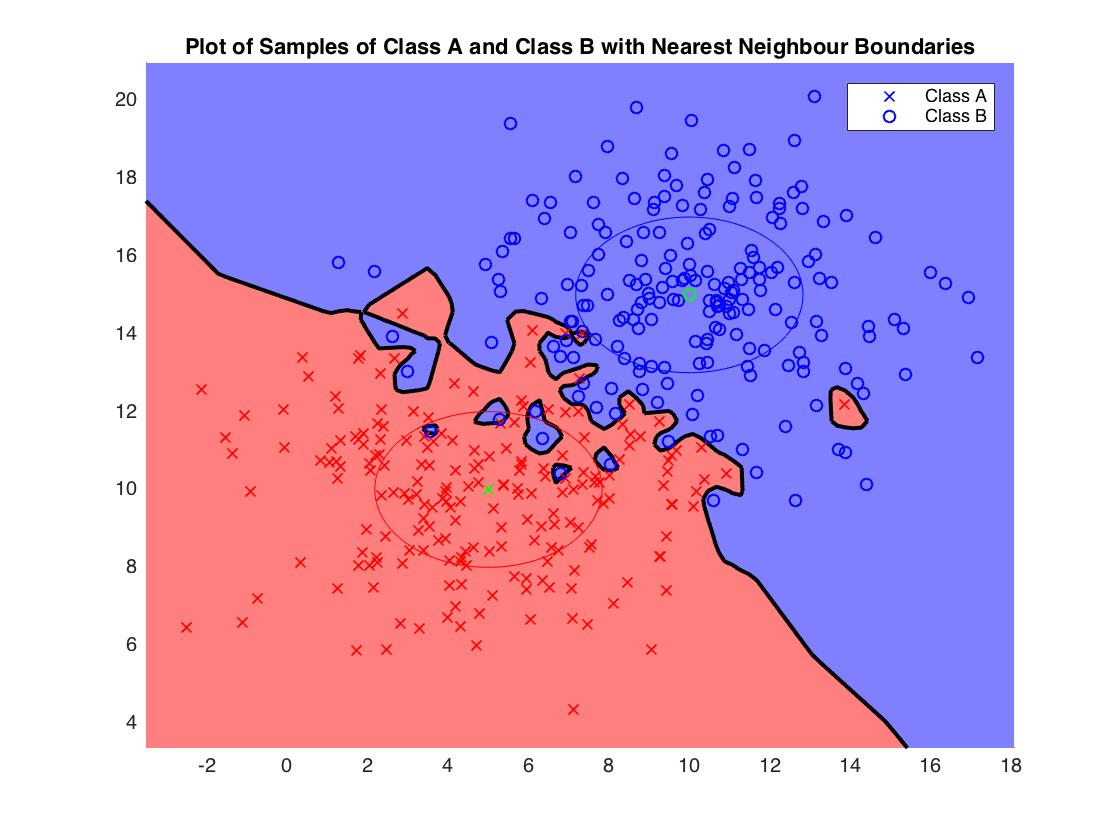
\includegraphics[width=0.5\textwidth]{case1_NN}
\label{fig:Case1_NN}
\end{figure}

Unlike the previous classifiers, the NN decision boundary is much more precise, and accounts for the outliers within the two sample classes. However, it's interesting to note that the boundary itself is not contiguous; there are smaller island-like sub-boundaries that form around the extreme outliers in either sample class.

In order to conduct an error analysis for the NN and kNN approaches, testing data needs to be generated to offset NN's reliance to overfit on training data. The testing data is created by using a new seed in the randomizing function and applying it to the \verb|bivariate_normal| function.

The experimental error rate for case 1 with the testing data was:
\begin{equation}
    P(\epsilon) = 0.0950
\end{equation}

The confusion matrix for Case 1 is summarized below:
\begin{table}[H]
    \centering
    \begin{tabular}{c|c c|c|}
        & \multicolumn{2}{c|}{\textbf{Predicted}} \\
        \textbf{Actual} & \textbf{A} & \textbf{B} & \textbf{Totals} \\
        \hline
        \textbf{A} & 177 \cellcolor[gray]{.8} & 23 & 200\\
        \textbf{B} & 15 & 185 \cellcolor[gray]{.8} & 200\\\hline
        \textbf{Totals} & 192 & 208\\
        \cline{1-3}
    \end{tabular}
    \caption{Confusion Table for Case 1 with NN}
    \label{tab:Case1_NN_error}
\end{table}

Case 2 has 3 classes instead of 2, with decision boundaries computed between all three pairs of classes. Similar to Case 1, the NN classifier is much more precise than the other classifiers, however, there still are islands of sub-boundaries.

\begin{figure}[H]
\caption{Plot of Case 2 with NN Classifier (Black Curves)}
\centering
\includegraphics[width=0.5\textwidth]{case2_NN}
\label{fig:Case2_NN}
\end{figure}

The experimental error rate was again determined in a similar fashion to Case 1: separate testing data was created using the same parameters as the training data but with a different random seed. The error rate was:

\begin{equation}
    P(\epsilon) = 0.2400
\end{equation}

The confusion matrix for Case 2 is shown below:
\begin{table}[H]
    \centering
    \begin{tabular}{c|c c c|c|}
        & \multicolumn{3}{c|}{\textbf{Predicted}} \\
        \textbf{Actual} & \textbf{C} & \textbf{D} & \textbf{E} & \textbf{Totals} \\
        \hline
        \textbf{C} & 64 \cellcolor[gray]{.8} & 5 & 31 & 100 \\
        \textbf{D} & 1 & 176 \cellcolor[gray]{.8} & 23 & 200\\
        \textbf{E} & 23 & 25 & 102 \cellcolor[gray]{.8} & 150\\\hline
        \textbf{Totals} & 88 & 206 & 156\\
        \cline{1-4}
    \end{tabular}
    \caption{Confusion matrix for Case 2 with NN}
    \label{tab:Case2_NN_error}
\end{table}

The kNN approach takes the same underlying implementation, but instead of using the single nearest neighbors for each class, it takes the $k$ nearest neighbors and generates a prototype based on the sample mean of the nearest neighbors. For the purposes of this lab, $k = 5$. These mean neighbors for each class are used then used to determine the decision boundary.The kNN classifier attempts to mitigate the overfitting in the NN classifier through the mean neighbor approach. Below is the decision boundary for Case 1 generated by the kNN classifier:

\begin{figure}[H]
\caption{Plot of Case 1 with kNN Classifier (Black Curves)}
\centering
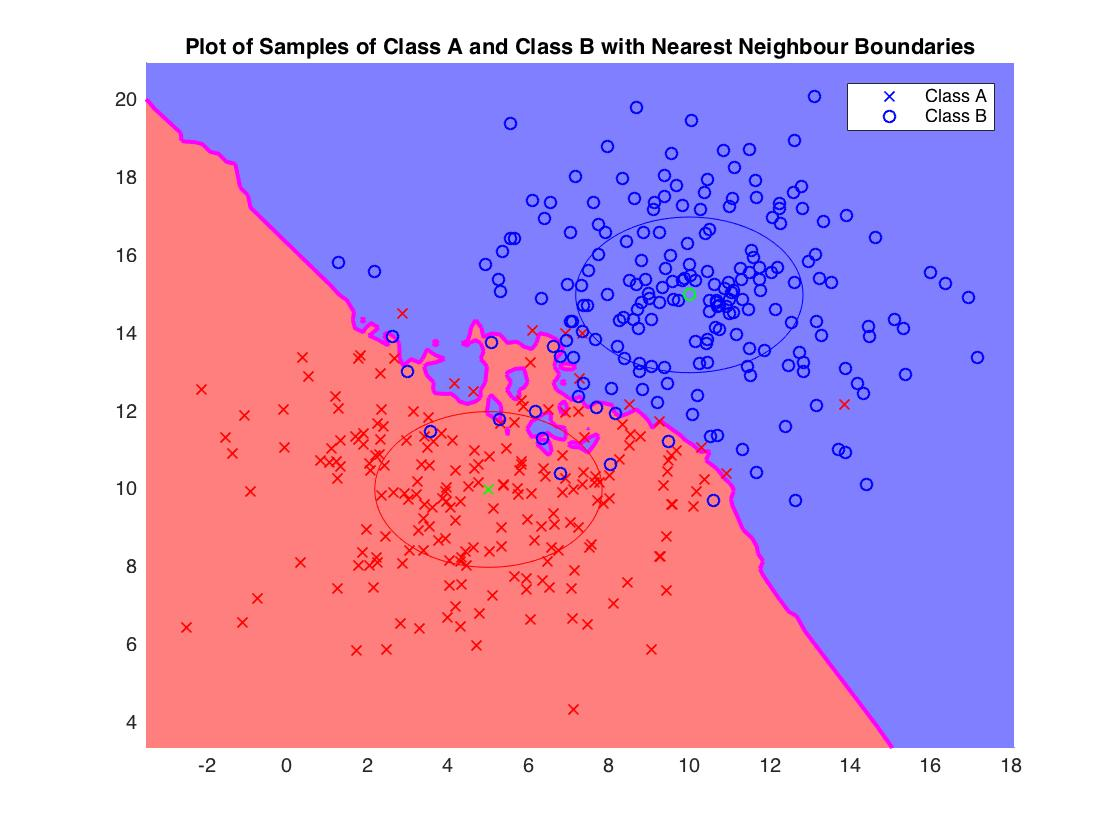
\includegraphics[width=0.5\textwidth]{case1_KNN}
\label{fig:Case1_KNN}
\end{figure}

Comparing Figures \ref{fig:Case1_NN} and \ref{fig:Case1_KNN}, it is clear that the kNN classifier reduces the overfitting and smooths out the resulting decision boundary. Using mean sampling, many of the sub-boundaries are also eliminated. The experimental error rate for the kNN classifier is shown below:
\begin{equation}
    P(\epsilon) = 0.0750
\end{equation}

The decrease in error rate compared to the NN classifier can be attributed to the decrease in overfitting; the decision boundary is much more generalized and can account for variations in the sample classes. The confusion matrix for Case 1 is shown below:

\begin{table}[H]
    \centering
    \begin{tabular}{c|c c|c|}
        & \multicolumn{2}{c|}{\textbf{Predicted}} \\
        \textbf{Actual} & \textbf{A} & \textbf{B} & \textbf{Totals} \\
        \hline
        \textbf{A} & 179 \cellcolor[gray]{.8} & 21 & 200\\
        \textbf{B} & 9 & 191 \cellcolor[gray]{.8} & 200\\\hline
        \textbf{Totals} & 188 & 212\\
        \cline{1-3}
    \end{tabular}
    \caption{Confusion Table for Case 1 with kNN}
    \label{tab:Case1_KNN_error}
\end{table}

Similar to Case 1, the kNN decision boundary for Case 2 is more generalized and has less islands or sub boundaries (see Figures \ref{fig:Case2_NN} and \ref{fig:Case2_KNN}).

\begin{figure}[H]
\caption{Plot of Case 2 with kNN Classifier (Black Curves)}
\centering
\includegraphics[width=0.5\textwidth]{case2_KNN}
\label{fig:Case2_KNN}
\end{figure}

The experimental error rate is again less than the NN classifier equivalent:
\begin{equation}
    P(\epsilon) = 0.2156
\end{equation}

The confusion matrix provides a more detailed view of the classification and resulting errors:

\begin{table}[H]
    \centering
    \begin{tabular}{c|c c c|c|}
        & \multicolumn{3}{c|}{\textbf{Predicted}} \\
        \textbf{Actual} & \textbf{C} & \textbf{D} & \textbf{E} & \textbf{Totals} \\
        \hline
        \textbf{C} & 65 \cellcolor[gray]{.8} & 4 & 31 & 100 \\
        \textbf{D} & 2 & 182 \cellcolor[gray]{.8} & 16 & 200\\
        \textbf{E} & 23 & 21 & 106 \cellcolor[gray]{.8} & 150\\\hline
        \textbf{Totals} & 90 & 207 & 153\\
        \cline{1-4}
    \end{tabular}
    \caption{Confusion matrix for Case 2 with kNN}
    \label{tab:Case2_KNN_error}
\end{table}


\section{Performance Comparison of Classifiers}
Each classifier was, to a degree, able to correctly assign classes. The decision boundaries of each classifier overlaid on one another show the differences (or lack thereof) in their predictions. They also show the strengths and weaknesses of each classifier and demonstrate the power of a classifier when it is able to leverage all of the information stored within a class prototype.

\subsection{Case 1}
The decision boundaries for each distance based classifier can be viewed together in figure \ref{fig:Case1_dist}. As is expected the MED classifier simply drew a line that is a perpendicular bisector to the line between each class prototype. However, both the GED and MAP classifiers gave identical decision boundaries. This is due to the fact that each class prototype contained the same covariance matrix and number of samples (i.e. same prior probabilities) meaning the MAP classifier simplified to the GED classifier. If more unit contours were plotted for each class, the GED/MAP line would go through the intersection of the unit contours of the two classes.

\begin{figure}[H]
    \caption{Plot of MED (magenta), GED (cyan) and MAP (black) decision boundaries for Case 1.}
    \centering
    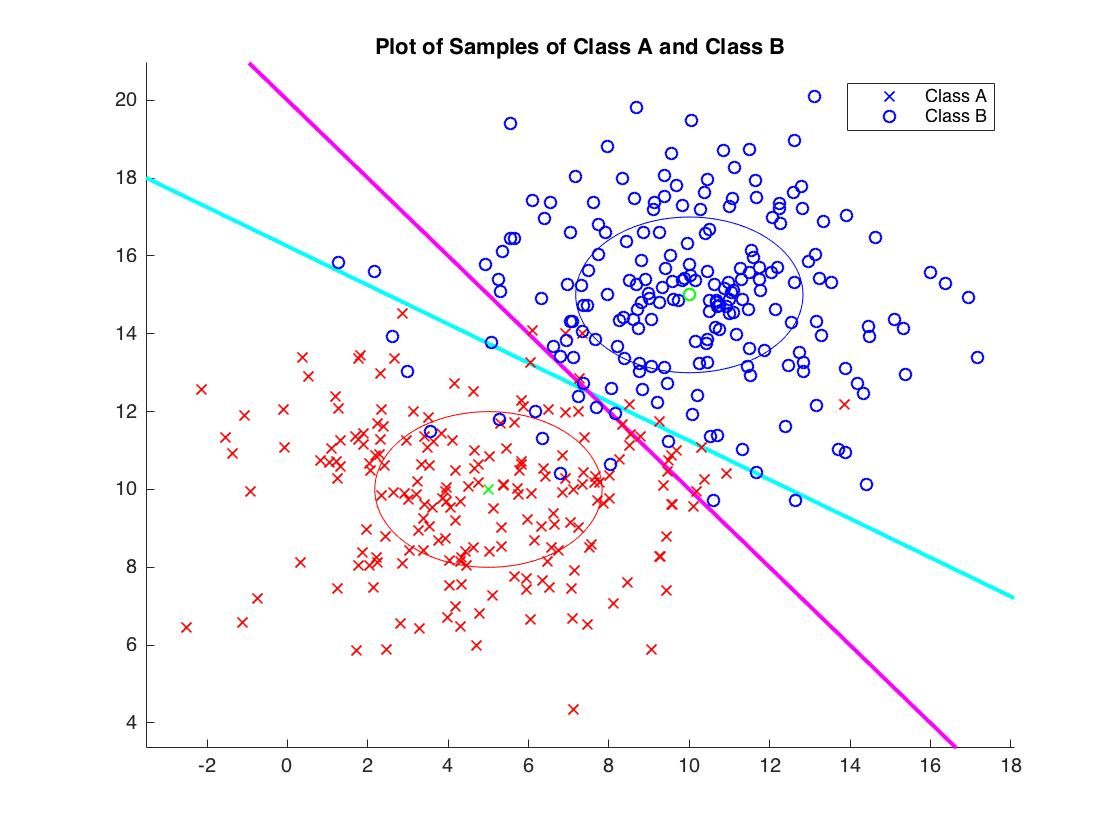
\includegraphics[width=0.5\textwidth]{Case1_dist_all}
    \label{fig:Case1_dist}
\end{figure}

As mentioned in Section 3.4, the NN and kNN classifiers create much more precise decision boundaries compared to the previous methods. However, the NN classifier leads to overfitting, where extreme values within the sample classes are accounted for and have their own sub-boundaries. This can be seen in Figure \ref{fig:Case1_nay_nay}, where there are distinct black sub-boundaries separate from the primary boundaries. The use of sample mean in the kNN classifier mitigates this, reflected in the much smoother magenta decision boundary, which has very few sub-boundaries.

\begin{figure}[H]
    \caption{Plot of NN (black) and kNN (magenta) decision boundaries for Case 1.}
    \centering
    \includegraphics[width=0.5\textwidth]{Case1_nay_nay_all}
    \label{fig:Case1_nay_nay}
\end{figure}

Overall for case 1, the MAP/GED classifiers had the lowest error rate of 0.0550. For a simple case with classes with equal variances, the simpler GED classifier performs just as well as MAP.

\subsection{Case 2}
The decision boundaries for each distance based classifier can be viewed in figure \ref{fig:Case2_dist}. Here the MED classifier performed poorly as each decision boundary was simply a line between the class prototypes. This behaviour was expected because the MED classifier simply measures the Euclidean distance between a point and the class prototype. The GED classifier behaved as expected by creating a non-linear decision boundary. This boundary passed through any intersection of the standard deviation contours and nicely between classes $D$ and $E$. Finally, as expected, the MAP classifier performed the best. This was due to the fact that the MAP classifier was able to take into account every feature of the class prototype the prior knowledge (number of samples) and the correlations of each class. This allowed the MAP classifier to perform optimally on the given data.

A noteworthy difference between the GED and MAP non-linear boundaries was how the MAP boundary between class $C$ and $E$ shifted left closer to class $C$. While the GED boundary is bound to the unit standard deviation contour, the MAP boundary is not, suggesting that it can better deal with overlapping classes.

\begin{figure}[H]
    \caption{Plot of MED (magenta), GED (cyan) and MAP (black) decision boundaries for Case 2}
    \centering
    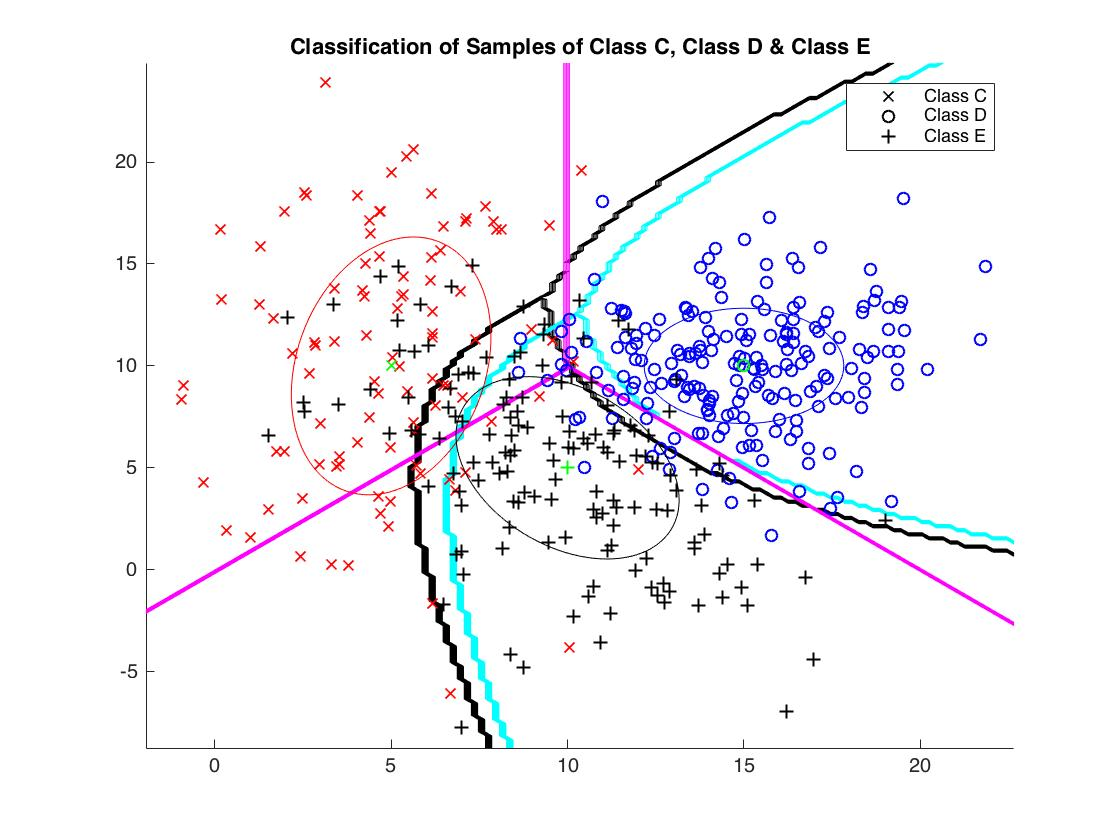
\includegraphics[width=0.5\textwidth]{Case2_dist_all}
    \label{fig:Case2_dist}
\end{figure}

Similar to Case 1, the decision boundary in Figure \ref{fig:Case2_nay_nay} drawn by the kNN implementation (magenta) is much smoother with less sub-boundaries due to the decrease in overfitting when compared to the NN classifier (black). This decrease in overfitting for the training data reflects in a better model; when the kNN classifier is applied to testing data, its resulting experimental error rate is less than its NN counterpart.

\begin{figure}[H]
    \caption{Plot of NN (black) and kNN (magenta) decision boundaries for Case 2}
    \centering
    \includegraphics[width=0.5\textwidth]{Case2_nay_nay_all}
    \label{fig:Case2_nay_nay}
\end{figure}

Overall for case 2, the MAP classifier had the lowest error rate of 0.1511 as it was the most powerful classifier and took advantage of all the information available including the variance, priors and volume of data. The NN and kNN approaches succumbed to overfitting, which led to high error rates.

From the confusion matrix of case 2 of all classifiers, it is apparent that class $E$ was often predicted incorrectly as class $C$ or $D$, whereas class $C$ and $D$ were rarely predicted as each other. This is mostly due to cluster $C$ and $D$ being relatively far apart while cluster $E$ sat right in between $C$ and $D$ and overlapped them significantly. Another interesting note from the confusion matrix was that the class with the most samples was always predicted more accurately.

\section{Conclusion}
One of the key takeaways from this lab was that the MAP classifier performed the best out of all classifiers tested against sample data. The MAP classifier, unlike the other classifiers discussed in this lab which rely on the Euclidean distance metric and variance, is also able to take the priors and volumes of each class' data into account when drawing the decision boundaries, thus improving its performance.

While the NN and kNN generally have the most precise decision boundaries for a given set of training data, they have a much higher error rate when applied to testing data due to their reliance to overfitting the training data.

\end{document}